\chapter{Implementación}
{\color{blue}



La implementación de la aplicación se realiza con \textbf{Kaa IoT} tal y como se analizo anteriormente \ref{eleccion-framework}. Para empezar a usar el framework, hay que registrarse en sistema. Una vez registrados tendremos acceso a nuestro \textit{dashboard} \footnote{Hace referencia al cuadro de mandos al que tenemos acceso para interactuar con nuestro dispositivo y todas las posibles configuraciones}. En este capítulo se trata de mostrar una guía con la que se consiga conectar un dispositivo, recoger y enviar datos desde/hacia el dispositivo y mostrar las opciones que nos ofrece Kaa IoT como framework IoT. Para empezar, vamos a conectar nuestro primer dispositivo.

\begin{figure}[hb!]
    \centering
    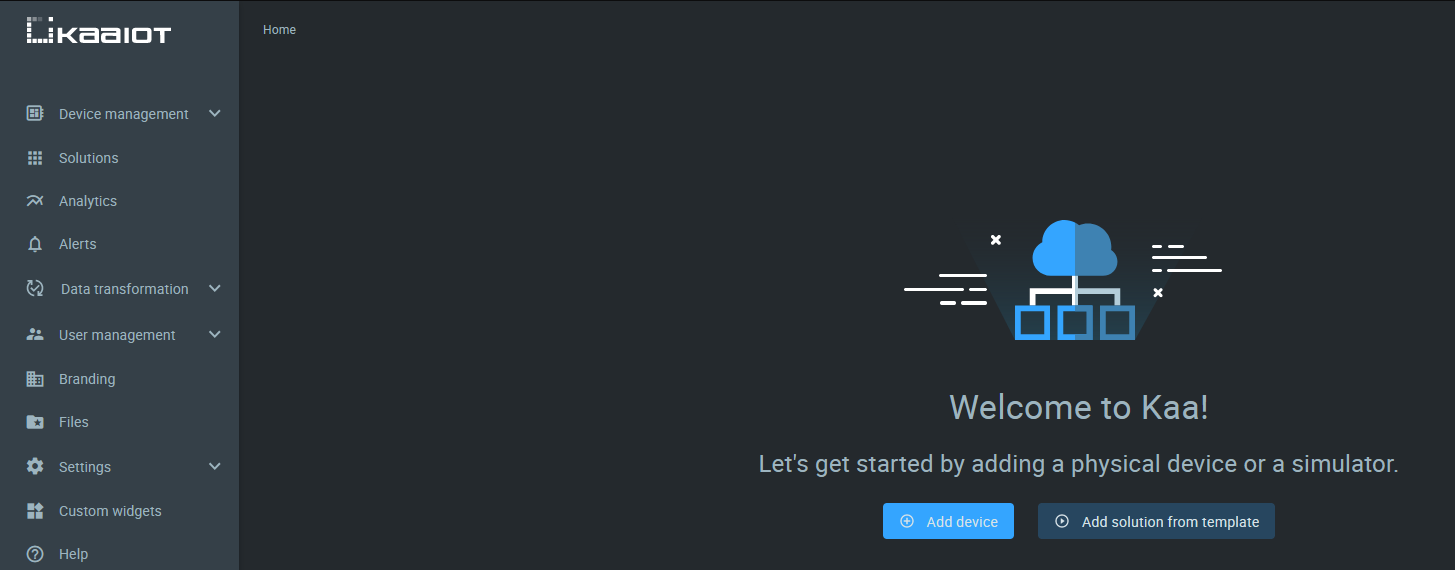
\includegraphics[width=\linewidth]{imagenes/dashboard.png}
    \caption{Dashboard Kaa IoT.}
    \label{fig:figure5}
\end{figure}


\section{Conectar dispositivo}

En este apartado se trata de explicar el proceso de conexión de un dispositivo con nuestra aplicación, desde crear un endpoint hasta ver la información del dispositivo en nuestra interfaz de usuario. Esto engloba varios términos y conceptos que se van a definir a continuación.

\subsection{Términos y conceptos}

\subsubsection{Endpoints}

Los endpoints representan ``el elemento de las cosas`` del IoT. Un endpoint es cualquier dispositivo terminal que se quiera gestionar, en nuestro caso desde Kaa IoT. Un endpoint puede ser un dispositivo físico o una emulación de software del mismo. Todos los datos que llegan a la aplicación están asociados a endpoints. \cite{kaaiotConcepts}

Para ser precisos, un endpoint puede ser una unidad menor que un dispositivo, lo que significa que un dispositivo físico puede incluir múltiples endpoints. Por ejemplo, quieres gestionar un termostato, para que el aire acondicionado se encienda y apague automáticamente a cierta temperatura.

Se puede gestionar el termostato de una de las siguientes maneras:

\begin{itemize}
    \item Toda la unidad del termostato actúa como un endpoint único que intercambia datos con el servidor.
    \item Los componentes del termostato, como los sensores de temperatura y humedad, interruptor de encendido/apagado, actúan como endpoints individuales.
\end{itemize}

\subsubsection{ID de Endpoint}

El ID de endpoints se utiliza para identificar de forma única un endpoint dentro de una instancia. Un ID de endpoints suele ser un UUID generado automáticamente por el framework en el momento de crear un nuevo endpoint. No obstante, también se permiten los ID de endpoints definidos por el usuario. El ID de los endpoints no puede modificarse una vez creado.

Todos los datos de los endpoints, como los atributos de los metadatos, los puntos de datos de series temporales recopilados, los comandos, etc., están asociados a un ID de endpoint específico. Siempre que recupere o gestione datos relacionados con endpoints en Kaa, principalmente a través de la API REST, se verá los ID de endpoints.

\subsubsection{Token del Endpoint}

Los tokens de endpoints se utilizan para la identificación de endpoints cuando se intercambian datos relacionados con los endpoints, utilizando los protocolos compatibles basados en MQTT y HTTP. Los tokens de endpoint son únicos dentro de una aplicación IoT y se asignan exactamente a un endpoint.

Cuando llega un mensaje de un cliente, el token del endpoint se resuelve en el correspondiente ID del endpoint. Un ejemplo sobre el protocolo MQTT, el token del endpoint va dentro de la llamada MQTT, por ejemplo:

\begin{lstlisting}[language=HTML]

kp1/<APPLICATION_VERSION>/epmx/<ENDPOINT_TOKEN>/get

\end{lstlisting}  \label{llamada-mqtt}

Normalmente, los tokens son cadenas generadas automáticamente por el framework, pero también se puede crear un token como el usuario quiera, por ejemplo, por el número de serie del dispositivo, dirección MAC, etc.

\subsubsection{Metadatos del endpoint}

Los metadatos de los endpoints son un conjunto de atributos clave-valor asociados a un endpoint. Se representan en el framework como un documento JSON de formato arbitrario.

Los metadatos de endpoints suelen incluir alguna información relacionada con los endpoints, como la ubicación, la descripción, el número de serie, la versión de hardware, etc. Los metadatos se almacenan en el servicio de registro de endpoints y pueden leerse o actualizarse de dos maneras:

\begin{itemize}
    \item A través de la capa de comunicación.
    \item A través de la API REST.
\end{itemize}

También se pueden gestionar los metadatos mediante la interfaz de usuario del framework.

\subsubsection{Aplicaciones y versiones}

Las aplicaciones en Kaa IoT sirven como contenedores para endpoints de diferentes tipos. Se puede tener una aplicación que contenga todos los endpoints que representan a un determinado dispositivo, y una aplicación para otro dispositivo, independiente de la otra aplicación. Las aplicaciones IoT también albergan toda la configuración del sistema necesaria para que el framework conozca las capacidades de sus dispositivos conectados y cómo trabajar con ellos.

Puede pasar que ya hemos configurado nuestro dispositivo, pero queremos implementar una nueva característica. Al implementarla se actualiza el firmware del dispositivo y se empieza a desplegar pero, ¿como diferenciamos entre los dispositivos que ya tienen el nuevo firmware y las que no? Aquí aparecen las versiones de una aplicación.

Cada aplicación puede tener varias versiones al mismo tiempo. Cada versión representa un conjunto de capacidades soportadas por los endpoints. En cualquier momento, cada endpoint está asociado a una versión de su aplicación. El conocimiento de la versión actual de la aplicación de un endpoint ayuda al framework a entender qué funcionalidad soporta el endpoint, cómo se formatean los datos, etc. Se puede utilizar las versiones para hacer evolucionar los dispositivos añadiendo o retirando funcionalidades mientras mantiene sus versiones antiguas en funcionamiento. Para diferenciar llamadas entre versiones se puede indicar como hemos visto en \ref{llamada-mqtt}.

\subsection{Pasos a seguir}

}

